% 指数を1減らすごとに値が半分になる図：2^3 から 2^{-2} まで（CC BY-SA 4.0）
\begin{tikzpicture}[xscale=1.1,yscale=0.42]
  \draw[->] (-0.3,0) -- (6.4,0);
  \foreach \i/\e/\v/\lab in {0/3/8/8, 1/2/4/4, 2/1/2/2, 3/0/1/1, 4/-1/0.5/\tfrac12, 5/-2/0.25/\tfrac14}{
    \ifnum\e<1 \def\barcol{red}\else \def\barcol{blue}\fi
    \fill[\barcol!55] (\i+0.15,0) rectangle (\i+0.85,\v);
    \node[above] at (\i+0.5,\v) {$\lab$};
    \node[below] at (\i+0.5,0) {$2^{\e}$};
  }
  \foreach \i in {0,...,4}{
    \draw[->,thick,black!60] (\i+0.6,-2.6) to[bend right=40] node[below=-1pt] {\scriptsize $\div 2$} (\i+1.4,-2.6);
  }
\end{tikzpicture}
